\documentclass[11pt,fleqn]{article}
\usepackage{graphicx}
\usepackage[letterpaper, margin=1in]{geometry}
\usepackage{hyperref}
\usepackage{mdframed}
\usepackage{amsmath}
\usepackage{caption}

\hypersetup{colorlinks=true, linktoc=all, linkcolor=blue}
\setlength{\parindent}{0pt}

\begin{document}

\begin{center}
\huge{\textbf{Stereo Vision Report}}\\[20pt]
\Large{Robert Washbourne}\\[20pt]
7911 Meadow Lake Lane, Houston, TX, 77063\\[20pt]
Washbourne Academy, Grade 9\\[20pt]
Last edited: \today
\end{center}

\newpage
\tableofcontents
\vspace{10pt}
\listoffigures
\newpage
\normalsize

\section{Abstract}

In August 2015, I began working on a project to find distances of objects using two webcams.  My initial interest in this project stemmed from seeing a video on self-driving cars. I thought that self-driving cars would need to somehow calculate distances to see how far away objects such as other cars are from them.\\[5pt]
%
Next I thought about the function of human vision and how our eyes perceive distance. We determine if objects are closer or farther away by comparing images from the left eye and the right eye. Based on human vision, my first project iteration used two cameras and compared each pixel from the camera images in order to generate a depth (distance) map.\\[5pt]
%
This pixel distance is added to a disparity matrix (a matrix full of pixel distances). Then, the disparity matrix distances are triangulated using the distance between the cameras. This matrix of distances can be converted to a 3D model.\\[5pt]
This method is fast enough to work in real time, and is what I am presenting in April 2016. The demonstration I have prepared utilizes two webcams mounted two centimeters apart on a piece of wood, and can resolve the depth of objects that are farther than three feet away. Future iterations of my project will include a faster algorithm, and the addition of creating 3-D models for scanning objects.


% ................................................
\newpage
\section{Introduction}
% ................................................

Imagine driving in the dark, alert but not noticing a deer crossing the road right in front of you. Using stereo vision methods to see what is close, your car could detect the deer and brake before you even notice the obstacle. Stereo cameras could find distances, and sensing something closer than 20 feet, send the location to a computer controlling the car. The computer could reason that driving into the obstacle would be catastrophic and turn on the brakes. The deer, and you, would be safe.

\subsection{What is stereo vision}

Stereo vision is a topic in computer vision where two images, taken from aligned cameras several centimetres apart, are processed and depth data is returned. For example, taking two images and using a simple algorithm, a grayscale image is returned, with lighter pixels indicaring smaller distance than darker pixels. This type of image is called a \texttt{disparity map}. With proper normalization, a \texttt{disparity map} can be turned into a \texttt{depth map}. See Figure \ref{fig:example1} for an example of a disparity map.

\begin{figure}[!h]
\begin{mdframed}
\centering
\setlength\tabcolsep{0.005\textwidth}
\begin{tabular}{ccc}
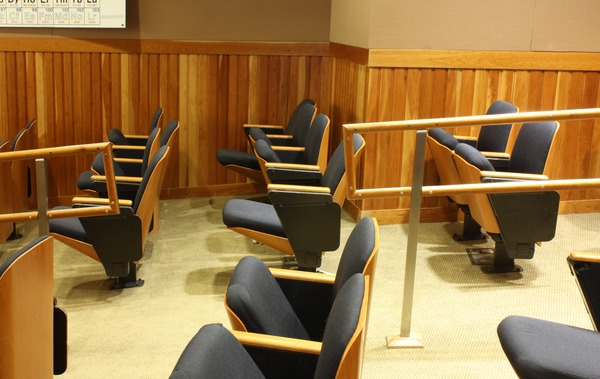
\includegraphics[width=0.32\textwidth]{images/im0-600.jpg} &
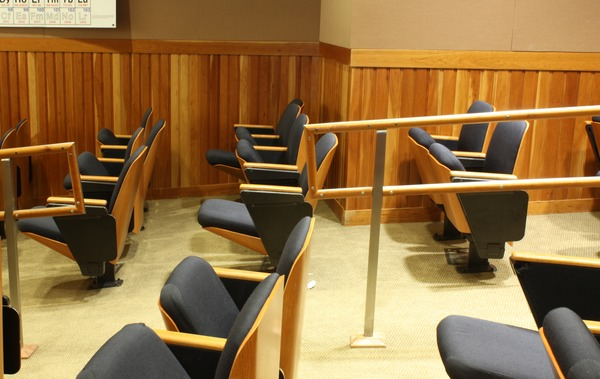
\includegraphics[width=0.32\textwidth]{images/im1-600.jpg} &
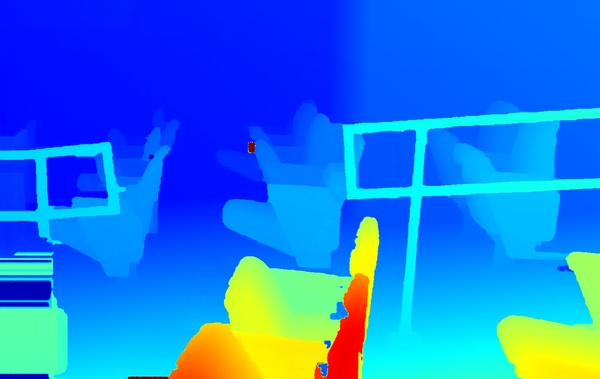
\includegraphics[width=0.32\textwidth]{images/disp-600.jpg} \\[2pt]
a) & b) & c)
\end{tabular}
\caption[Example of stereo vision]{Example of stereo vision: a) Image from left camera. b) Image from right camera c) Disparity map mapwhere the colors correlate with distance, with cool colors (blue) far away and hot colors (red) close.}
\label{fig:example1}
\end{mdframed}
\end{figure}


% ................................................
\section{Project Details}
% ................................................

Following are descriptions of the workflow steps required in order to perform stereo vision and generate \texttt{disparity maps} in real time.

\subsection{Calibrate stereo webcams}
When taking pictures for stereo vision, you need to make sure that the cameras are aligned exactly vertically and horizontally. If they aren't, the disparity map is noisy. I invested considerable time in aligning my cameras to improve the results of the disparity mapping.\\[5pt]
%
Once the cameras are physically aligned, you can calibrate them. To calibrate two cameras, you print a picture of a chessboard, and using an algorithm called SIFT key point detection, find the corners of the chessboard in both photos. SIFT is a method to detect edges in images. \\[5pt]
%
\newpage
Once you have the corners as key points, you can find the transformation matrix that maps from the left image to the right image. Using this transformation matrix, the cameras can be perfectly centered, therefore making better disparity maps with less noise.

\subsection{Capture images from stereo webcams}
My setup is a wooden board with 2 Microsoft LifeCam 3000 webcams mounted 2 centimeters apart, facing the same direction. This configuration can capture images of anything farther than three feet away, and works indoors and outdoors. Figure \ref{fig:cam} below is a photograph of my webcam setup.\\

\begin{figure}[!h]
\begin{mdframed}
\centering
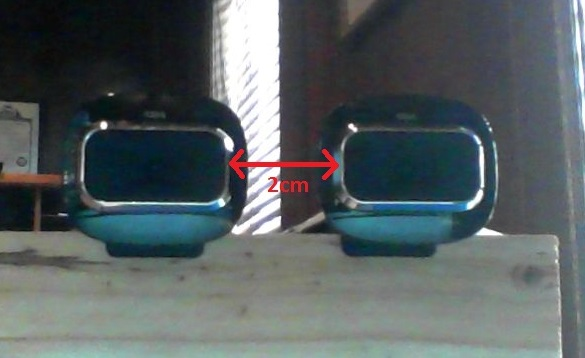
\includegraphics[width=0.85\textwidth, trim=30 50 45 50, clip]{images/setup.jpg}
\caption[Photo of the stereo webcams used for real time processing]{Photo of the left and right stereo webcams used for real time processing}
\label{fig:cam}
\end{mdframed}
\end{figure}

Figure \ref{fig:image1} shows two images of me in captured from the webcams. To see the results for these images, refer to Figure \ref{fig:image2}.
This is a picture of me, from about 10 feet away.\\

\begin{figure}[!h]
\begin{mdframed}
\centering
\setlength\tabcolsep{0.005\textwidth}
\begin{tabular}{cc}
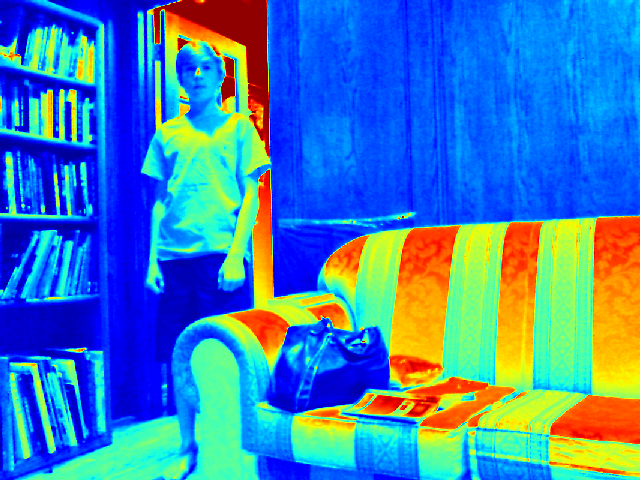
\includegraphics[width=0.45\textwidth]{images/l.png} &
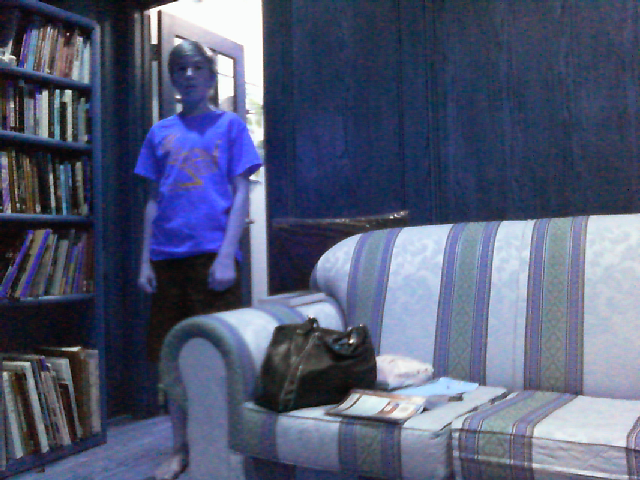
\includegraphics[width=0.45\textwidth]{images/r.png} \\[2pt]
\end{tabular}
\caption[Example images captured from webcams]{Example images captured from left and right webcams.}
\label{fig:image1}
\end{mdframed}
\end{figure}

\subsection{Split images into one pixel high rows and correlate}

Figure \ref{fig:strips} below is a comparison of the intensity from a single row near the bottom of the images shown in Figure \ref{fig:example1}. You can observe that the data from the left image (red line) is shifted by approximately 60 pixels towards the right with respect to the data from the right image (blue line).\\[5pt]
%
In other words, if you shift the red line about 60 pixels towards the left, it will line up quite well with the blue line. If you compare the two figures, you can observe that the apparent shift in the intensity values (Figure \ref{fig:strips}) is consistent with the apparent shift in the two images (Figure \ref{fig:example1}). \\[5pt]
%
For each output pixel in the correlation, a window is slid along the right image's row to find a match for that pixel with the left image. If we did this for the 100th pixel of the blue line in Figure 2, we would find that the corresponding red point is approximately 60 pixels to the right.\\

\begin{figure}[!h]
\begin{mdframed}
\centering
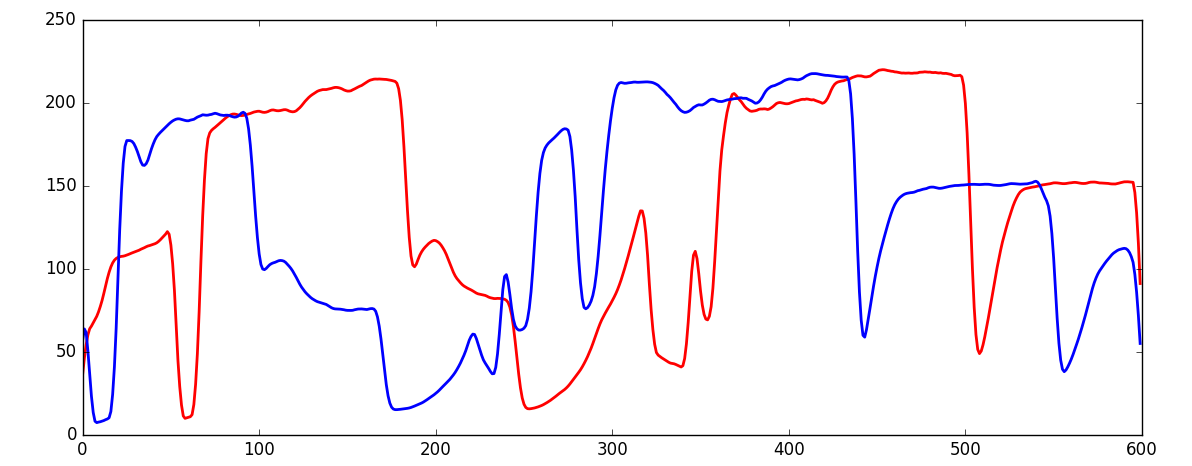
\includegraphics[width=1\textwidth]{images/strips.png} \\[2pt]
\caption[Intensity of the one pixel strips taken from the images in Figure \ref{fig:example1}]{Magnitude of one pixel strips from the images in Figure \ref{fig:example1}. The row from the left image is shown with the blue line, and the row from the right image is shown with the red line. The horizontal axis is the column index from the images shown in Figure \ref{fig:example1}, and the vertical axis is the intensity value at that location. For example, at column 300 the left image intensity (blue line) is approximately 200.}
\label{fig:strips}
\end{mdframed}
\end{figure}

\subsection{Estimate pixel distance}
The pixel distance that we find via correlation is added to the relevant output row and column of the \texttt{disparity map}.

\subsection{Apply edge preserving median filter}

The disparity maps produced by this technique can be noisy, and we apply filtering in order to reduce the noise.\\[5pt]
%
A median filter works by applying a particular type of edge preserving averaging to pixels. Median filtering is quite simple, requiring two steps per output location:

\newpage
\begin{enumerate}
\item sort the samples in the input window by magnitude
\item take the median sample value as the output value
\end{enumerate}
%
In order to show the meaning and usefulness of median filters, Figure \ref{fig:median_illustrate} below illustrates the application of a median filter to random image data, and Figure \ref{fig:medians} shows a median filter applied to real disparity map data.\\

\begin{figure}[!ht]
\small
\begin{mdframed}
\begin{equation*}
\begin{aligned}
&\texttt{4x4 section of representative input image data}\\
& \hspace{20pt} \begin{bmatrix}
2 & 0 & 3 & 5 \\
1 & 4 & 2 & 7 \\
3 & 1 & 0 & 3 \\
6 & 8 & 4 & 2 \\ 
\end{bmatrix} \\[10pt]
%
& \texttt{Application of 3x3 median filter to the $(2,2)$ interior filter location}\\
& \hspace{20pt} \begin{bmatrix}
\mathbf{2} & \mathbf{0} & \mathbf{3} & 5 \\
\mathbf{1} & \mathbf{4} & \mathbf{2} & 7 \\
\mathbf{3} & \mathbf{1} & \mathbf{0} & 3 \\
6 & 8 & 4 & 2 \\ 
\end{bmatrix} 
\rightarrow (2, 0, 3, 1, 4, 2, 3, 1, 0) \rightarrow (0, 0, 1, 1, 2, 2, 3, 3, 4) \rightarrow (2) \\[10pt]
%
& \texttt{Application of 3x3 median filter to the $(2,3)$ interior filter location}\\
& \hspace{20pt} \begin{bmatrix}
2 & \mathbf{0} & \mathbf{3} & \mathbf{5} \\
1 & \mathbf{4} & \mathbf{2} & \mathbf{7} \\
3 & \mathbf{1} & \mathbf{0} & \mathbf{3} \\
6 & 8 & 4 & 2 \\ 
\end{bmatrix} 
\rightarrow (0, 3, 5, 4, 2, 7, 1, 0, 3) \rightarrow (0, 0, 1, 2, 3, 4, 4, 5, 7) \rightarrow (3) \\[10pt]
%
& \texttt{Application of 3x3 median filter to the $(3,2)$ interior filter location}\\
& \hspace{20pt} \begin{bmatrix}
2 & 0 & 3 & 5 \\
\mathbf{1} & \mathbf{4} & \mathbf{2} & 7 \\
\mathbf{3} & \mathbf{1} & \mathbf{0} & 3 \\
\mathbf{6} & \mathbf{8} & \mathbf{4} & 2 \\ 
\end{bmatrix} 
\rightarrow (1, 4, 2, 3, 1, 0, 6, 8, 4) \rightarrow (0, 1, 1, 2, 3, 4, 4, 6, 8) \rightarrow (3) \\[10pt]
%
& \texttt{Application of 3x3 median filter to the $(3,3)$ interior filter location}\\
& \hspace{20pt} \begin{bmatrix}
2 & 0 & 3 & 5 \\
1 & \mathbf{4} & \mathbf{2} & \mathbf{7} \\
3 & \mathbf{1} & \mathbf{0} & \mathbf{3} \\
6 & \mathbf{8} & \mathbf{4} & \mathbf{2} \\ 
\end{bmatrix} 
\rightarrow (4, 2, 7, 1, 0, 3, 8, 4, 2) \rightarrow (0, 1, 2, 2, 3, 4, 4, 7, 8) \rightarrow (3) \\[10pt]
%
& \texttt{Output 3x3 median filtered data, with edge locations zeroed}\\
& \hspace{20pt} \begin{bmatrix}
0 & 0 & 0 & 0 \\
0 & 2 & 3 & 0 \\
0 & 3 & 3 & 0 \\
0 & 0 & 0 & 0 \\ 
\end{bmatrix}
\end{aligned}
\end{equation*}
\caption[Illustration of median filter application]{Illustration of median filter application.}
\label{fig:median_illustrate}
\end{mdframed}
\end{figure}

\begin{figure}[!h]
\begin{mdframed}
\centering
\begin{tabular}{cc}
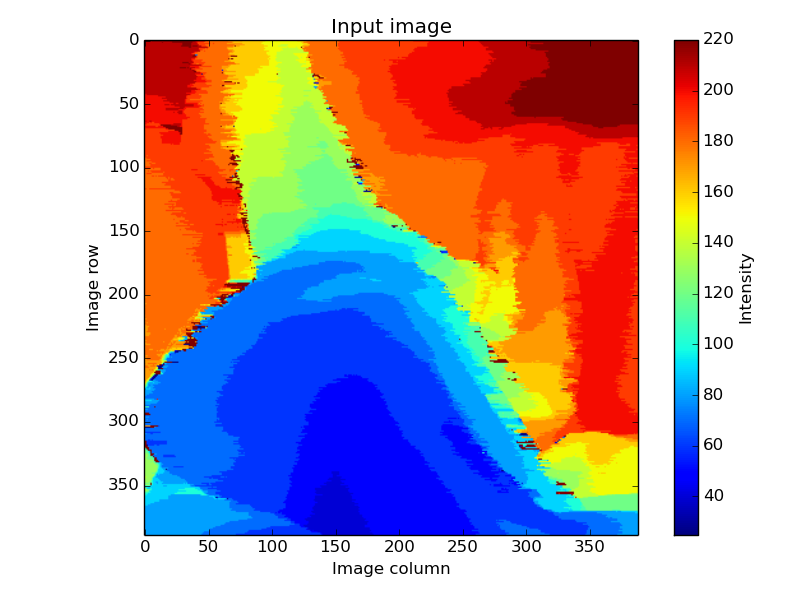
\includegraphics[width=0.49\textwidth, trim=60 10 25 10, clip]{images/median1.png} &
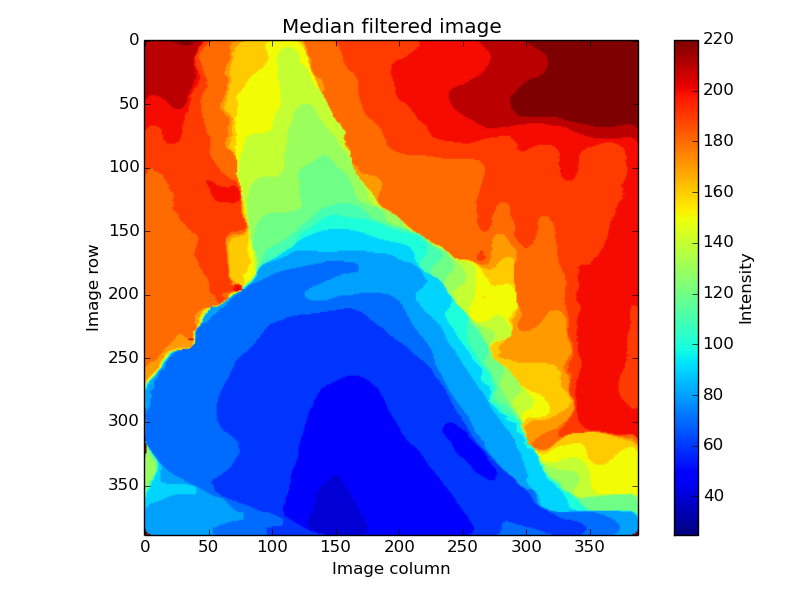
\includegraphics[width=0.49\textwidth, trim=60 10 25 10, clip]{images/median2.png}\\[2pt]
a) & b) \\
\end{tabular}
\caption[Example of 11x11 median filter applied to disparity map]{Example of 11x11 median filter applied to disparity map where the colors correlate with distance, with cool colors (blue) are far away and hot colors (red) close. a) Before median filter b) After median filter. 
The noise reducing effects of a median filter are evident.}
\label{fig:medians}
\end{mdframed}
\end{figure}


\subsection{Return the final disparity map}

The output disparity map has values that do not show distance. To turn these values into distance, the program triangulates using the distance between cameras.\\[5pt]
%
There are several methods of creating disparity maps. They can be created by a laser scanner, but this process is much slower than stereo matching and unsuited for real time processing. \\[5pt]
%
Disparity maps can also be created with two cameras. This is the method that I explored, and it is fast enough for real time processing and yields acceptable results. In images created with this technique, a colormap is used to make it easier to see what is closer.\\[5pt]
%
Figure \ref{fig:result1} compares results for the laser and stereo vision approaches, from the Middlebury Computer Vision dataset. The laser result is crisper, but it takes much longer to generate. The stereo matching result is worse, with parts of the image blended, but it was generated much faster. \\

\begin{figure}[!h]
\begin{mdframed}
\centering
\setlength\tabcolsep{0.005\textwidth}
\begin{tabular}{ccc}
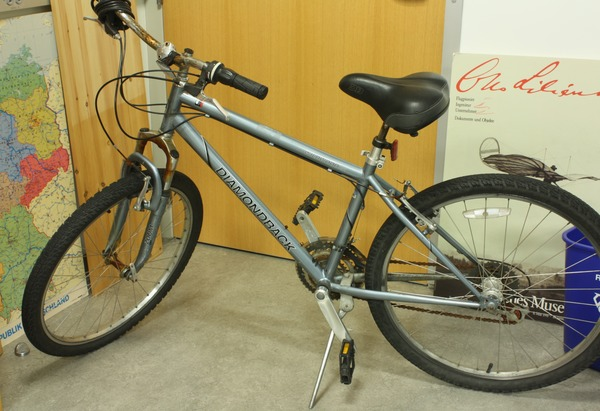
\includegraphics[width=0.3\textwidth]{images/_im0-600.jpg} &
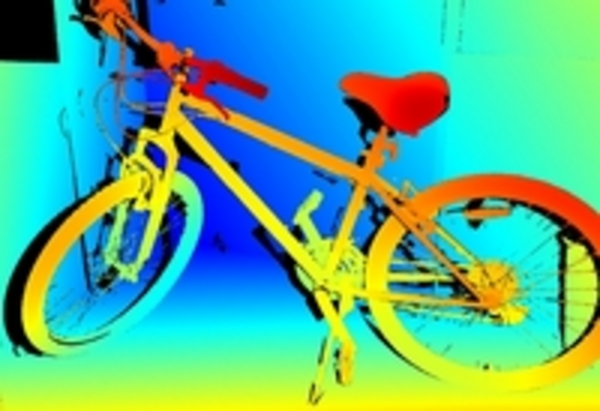
\includegraphics[width=0.3\textwidth]{images/disp0GT-600.jpg} &
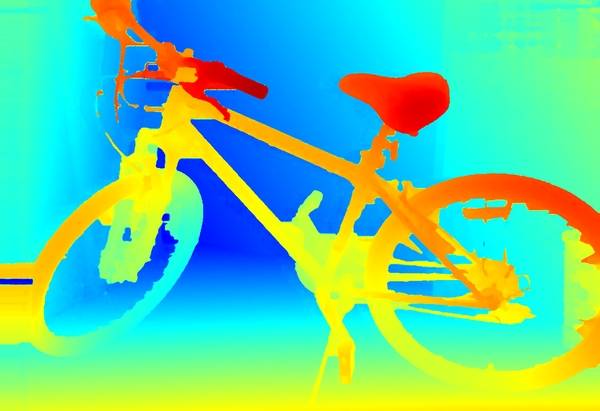
\includegraphics[width=0.3\textwidth]{images/_disp-600.jpg} \\[2pt]
\end{tabular}
\caption[Comparison of laser and stereo derived disparity maps]{Comparison of laser and stereo derived disparity maps: left) Original image center) Laser result right) Disparity Matching result.}
\label{fig:result1}
\end{mdframed}
\end{figure}

\newpage
Figure \label{fig:image2} shows  results from my experiment, taken with web cams I mounted and calibrated. See Figure \ref{fig:cam} for details about my stereo vision setup.\\

\begin{figure}[!h]
\begin{mdframed}
\centering
\setlength\tabcolsep{0.005\textwidth}
\begin{tabular}{cc}
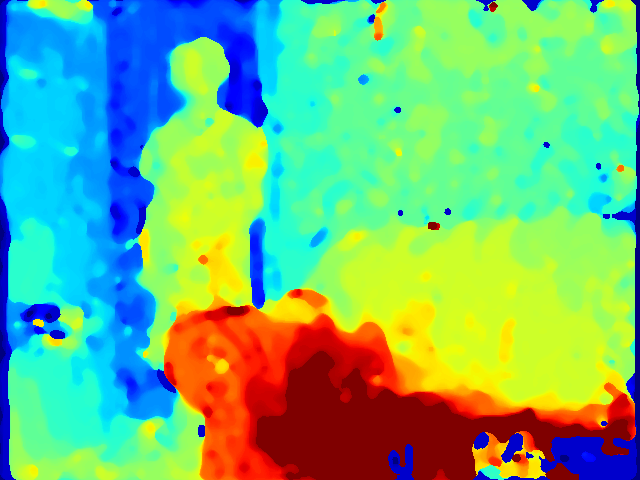
\includegraphics[width=0.45\textwidth]{images/res.png} &
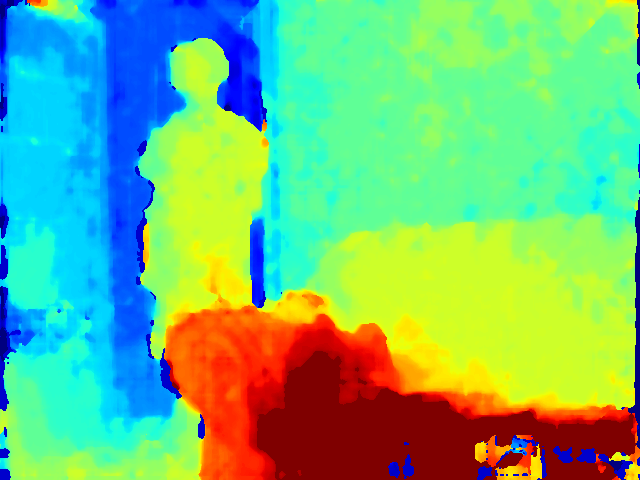
\includegraphics[width=0.45\textwidth]{images/nomedres.png} \\[2pt]
a) & b) \\
\end{tabular}
\caption[Results from my setup]{Results from my setup for the left and right camera images shown in Figure \ref{fig:image1}. The colors correlate with distance, where cool colors (blue) are far away and hot colors (red) are close. a) Raw disparity map b) Median filtered disparity map.}
\label{fig:image2}
\end{mdframed}
\end{figure}

\section{Discussion}

\subsection{Optimization of performance}

It took me several months to get my implementation working, and once I did, it was not performing nearly fast enough to work in real time. To optimize performance, I wrote code for a special python video grabbing method that utilized multi-threading to capture new frames simultaneously as previous frames were being processed. This increased the \texttt{frames per second} of my webcams from 30 FPS to 60 FPS, making the project two times faster.\\[5pt]
%
In addition, each row of the image is processed by a different thread, effectively making the code run approximately 10 times faster.

\subsection{Applications}

stereo vision has many applications in computer science and image processing. Some real world applications already being developed. The Intelligent Vehicles Symposium published a paper on an algorithm that does analysis of traffic and car tracking. Google and other autonomous car manufacturers use stereo vision to pilot their self driving cars, and avoid and sense obstacles.

\subsection{Future work}

In the future, I would like to further optimize the performance of the code, and  make higher quality depth maps using post processing methods (algorithms that work on the \texttt{disparity maps}). I would also like to combine my work on stereo vision with image tracking and face recognition to make a 3D tracking system that can detect faces and track their distance and direction of movement.


% ................................................
\section{Conclusion}
% ................................................

Disparity maps can be used for many things: traffic control, autonomous cars, and even 3D models. But the main interest of stereo vision is just how cool it is. Using stereo vision, computers can tell how far away objects are, and detect obstacles. Stereo vision can make vehicles, drones, and toys smart and sense objects better. I thought that stereo vision would be much easier than it was, but I am glad that it was hard, because I learned a lot and had a lot of fun.


% ................................................
\section{Acknowledgements}
% ................................................

I would like to acknowledge several people for monitoring my project, explaining several formulas and giving feedback.\\[5pt]
%
As my science teacher, Dr. Dedra Demaree gave me valuable feedback on my results.\\[5pt]
%
Dr. John Washbourne, my dad, is a professional research engineer, has helped me learn LaTeX, program the median filter, and appreciates the engineering aspects of this project.


% ................................................
\section{References}
% ................................................

\begin{enumerate}
\item Joos, Franke U. "Real-time Stereo Vision for Urban Traffic Scene Understanding." IEEE Xplore. Intelligent Vehicles Symposium, 2 Apr. 2000. Web. 02 Apr. 2016.
\item Middlebury Computer Vision dataset for the example images and laser vs stereo matching comparison.  
\small
http://vision.middlebury.edu
\normalsize

\item Images used in figure \ref{fig:example1}\\  
\small
http://vision.middlebury.edu/stereo/datasets3/test/Classroom2/im0-600.jpg\\
http://vision.middlebury.edu/stereo/datasets3/test/Classroom2/im1-600.jpg\\
http://vision.middlebury.edu/stereo/results3/outputs/alg0034/test/Classroom2/disp-600.jpg
\normalsize

\item Images used in figure \ref{fig:result1}\\  
\small
http://vision.middlebury.edu/stereo/datasets3/test/Bicycle2/im0-600.jpg\\
http://vision.middlebury.edu/stereo/datasets3/test/Bicycle2/disp0GT-600.jpg\\
http://vision.middlebury.edu/stereo/results3/outputs/alg0034/test/Bicycle2/disp-600.jpg
\normalsize
\end{enumerate}

\end{document}

